\section{设计背景}
\subsection{设计任务背景}
% 本次设计服务对象为四川某城市,设计污水厂类型为城镇污水处理厂。四川
% 某城市位于成都平原,污水收集范围包括主城区大部分、城西镇工业小区、经济
% 开发区期地块、城东居住区及国际商贸部分地块,总建设用地面积为 133 km$^2$。
% 该市排水系统采用完全分流制体制,经过多年的开发建设,逐步形成了主城区的
% 污水系统,并已初具规模,现有城区排水管道 40530 m。

本次设计任务的服务对象为四川某城市,设计的目标是建设一个城镇污水处理厂。该城市位于成都平原,涵盖了主城区的大部分地区,城西镇的工业小区,经济开发区的待开发地块,城东的居住区以及国际商贸部分地块。总的建设用地面积为133平方千米。

目前,该城市的排水系统采用完全分流制体制,经过多年的开发建设,已初具规模。现有城区排水管道长度为40530米。
但随着城市的不断发展和人口的增加,该城市的污水处理需求日益迫切。因此,设计一个高效可靠的城镇污水处理厂是非常必要的。该污水处理厂的建设将为城市提供一个集中处理污水的设施,确保城市的水环境质量得到有效维护和改善。

% 设计任务的关键要求包括:
% \begin{enumerate}
% 	\item 处理能力:污水处理厂应具备足够的处理能力,能够满足城市当前和未来的污水处理需求。
% 	\item 技术先进性:采用先进的污水处理技术,确保出水质量符合相关标准,达到排放要求。
% 	\item 设计可行性:考虑到现有的城市排水系统,设计方案应与现有排水管道衔接良好,最大程度上减少对现有基础设施的改动。
% 	\item 可持续性:设计应考虑能源利用和废物处理等方面的可持续性,以最大程度地减少对环境的影响。
% 	\item 安全可靠性:设计应考虑设备运行的安全性和可靠性,确保污水处理过程稳定运行,减少事故风险。
% \end{enumerate}

通过本次设计任务,希望能够为该城市提供一个高效、可靠、环保的城镇污水处理厂,以改善城市的水环境质量,保护公众健康,促进城市的可持续发展。

% 该水厂所收纳的污水源很广泛,主体处理工艺为“预处理→厌氧池→卡鲁塞尔氧化沟→二沉池→消毒池”,设计出水标准执行《城镇污水处理厂污染物排放标准》(GB18918-2002)一级A类标准,和四川省生态环境厅在贴合国家政策的基础上出台的《四川省岷江、沱江流域水污染物排放标准》(DB51/2311-2016)规定。设计规模大于 35000 m$^3$/d 的城镇污水处理厂,从而有效地提高区域水环境质量,实现地表水污染治理目标。

\subsection{出水排放标准规范}
本次设计服务的对象是位于四川某城市的城镇污水处理厂。在设计城镇污水处理厂时,除了需要满足中华人民共和国国家标准《城镇污水处理厂污染物排放标准》(GB18918-2002)外,还必须符合该地区的地方标准,例如四川省地方标准《四川省岷江、沱江流域水污染物排放标准》(DB51/2311-2016)。

根据《城镇污水处理厂污染物排放标准》,污水处理厂的污水排放应符合一级标准、二级标准或三级标准。具体要求如下:
\begin{table}[H]
	\centering
	\caption{城镇污水处理厂污染物排放标准\cite{GB189182002}}
	\begin{tabular}{cccccc}
	\multicolumn{6}{r}{单位:mg/L} \\
	\toprule
	\multirow{2}[4]{*}{序号} & \multirow{2}[4]{*}{基本控制项目} & \multicolumn{2}{c}{一级标准} & \multirow{2}[4]{*}{二级标准} & \multirow{2}[4]{*}{三级标准} \\
	\cmidrule{3-4}          &       & A标准   & B标准   &       &  \\
	\midrule
	1     & 化学需氧量(COD) & 50    & 60    & 100   & 120 \\
	2     & 生化需氧量(BOD$_5$) & 10    & 20    & 30    & 60 \\
	3     & 悬浮物(SS) & 10    & 20    & 30    & 50 \\
	4     & 总氮(以N计) & 15    & 20    & -     & - \\
	5     & 氨氮(以N计)\footnotemark & 5(8)  & 8(15) & 25(30) & - \\
	6     & 总磷(以P计) & 0.5   & 1     & 3     & 5 \\
	7     & pH    & \multicolumn{4}{c}{6.0 $\sim$ 9.0} \\
	\bottomrule
	\end{tabular}
	\label{tab:Pollutant discharge standards for urban sewage treatment plants}%
\end{table}%
\footnotetext{括号外数值为水温 $>12$ ℃时的控制指标,括号内数值为水温 $\leqslant 12$ ℃时的控制指标。}

根据《四川省岷江、沱江流域水污染物排放标准》,不同类型的排污单位有特定的排放标准。对于城镇污水处理厂,其污水排放要求如下:

\begin{table}[H]
	\centering
	\caption{四川省岷江、沱江流域水污染物排放标准\cite{DB5123112016}}
	\resizebox{\textwidth}{!}{ % 调整表格的大小
	\begin{tabular}{ccccccc}
		\multicolumn{7}{r}{单位:mg/L} \\
		\midrule
		\multirow{2}[2]{*}{序号} & \multirow{2}[2]{*}{排污单位} & 化学需氧量 & 五日生化需氧量 & 氨氮    & 总氮    & 总磷 \\
				&       & (COD$\mathrm{_{C_r}}$) & (BOD$_5$) & (以N计) & (以N计) & (以P计) \\
		\midrule
		1     & 城镇污水处理厂 & 30    & 6     & 1.5(3) & 10    & 0.3 \\
		2     & 工业园区集中式污水处理厂 & 40    & 10    & 3(5)  & 15    & 0.5 \\
		3     & 规模化畜禽养殖场 & 100   & 30    & 25    & 40    & 3 \\
		4     & 制革及毛皮加工工业 & 50    & 20    & 15    & 20    & 0.5 \\
		5     & 纺织染整工业 & 60    & 15    & 10    & 15    & 0.5 \\
		6     & 合成氨工业 & 50    & 15    & 15    & 25    & 0.5 \\
		7     & 无机磷化学工业 & 40    & 20    & 10    & 15    & 5 \\
		8     & 有机磷类农药工业 & 50    & 20    & 10    & l5    & 10 \\
		\bottomrule
	\end{tabular}}
	\label{tab:Water pollutant discharge standards in the Minjiang and Tuojiang River basins of Sichuan Province}%
\end{table}%

通过满足国家和地方标准的要求,设计的城镇污水处理厂将能够有效地处理污水,并确保排放水质符合相关标准,保护环境和公众健康。


\subsection{设计目的及任务}

针对该污水处理厂水质水量的变化特征,我们在设计过程中充分考虑了进水结构的不平衡以及污泥负荷偏高等因素。我们综合参考了相关文献和工程实例,并综合考虑了实际难题,将所用到的资料都妥善插入到参考文献中。

为了确保该处理厂易于管理,并符合排放标准,我们选择了经过验证可靠运行的污水处理技术流程。我们详细计算了主要改建建筑物和设备的类型、数量以及主要建构物的平断面配置和位置。我们还考虑了设计尺寸的要求,并为实际建设选择了合适的材料,以确保符合规范。

在完成了技术设计平面布置和各设备的空间布置后,我们根据计算数据和相关规范绘制了相应的图面,以便清晰地呈现设计方案。

% 根据该污水处理厂水质水量的变化特征,充分考虑了当前进水结构的不平衡、污泥负荷偏高等特征,设计了该污水处理技术,在符合经济预算的前提下达到标准并排放。同时查阅相关文献,研究相关工程实例,充分考虑实际难题,根据排放标准易于管理,选择运行可靠的污水处理技术流程,确定主要改建建筑物和设备的类型和数量,确定主要建构物的平断面配置和位置,计算尺寸,选择使用材料为实际建设提供了规范的参考。完成技术设计平面布置和各设备的空间布置,提供经济概算,根据计算数据和相关规范绘制图面。




\newpage % 章节结尾换页

\section{设计总说明}
\subsection{工程概况}
\subsubsection{城市概况}
本次设计服务对象为四川某城市,位于成都平原,污水收集范围包括主城区大部分、城西镇工业小区、经济开发区期地块、城东居住区及国际商贸部分地块,总建设用地面积为 133 km$^2$。该市排水系统采用完全分流制体制,经过多年的开发建设,逐步形成了主城区的污水系统,并已初具规模,现有城区排水管道 40530 m。

\subsubsection{污水处理厂概况及设计规模}
\begin{enumerate}
	\item 污水厂类型:城镇污水处理厂。
	\item 总建设用地面积:133 km$^2$。
	\item 厂址东西向 600 m,南北宽 500 m,厂区设计地坪绝对标高为 498.00 m。
	\item 污水处理厂进水泵房污水进水管管底标高为 493.15 m,坡度 $1.0 \%$,充满度为 0.65。
	\item 海拔高度:$490\sim 520$,西北高,东南低。
	\item 气温:最冷月平均为 5 ℃,最热月平均为 32.5 ℃,最冷月水温在 $8\sim 12$ ℃取。
	\item 设计进水平均日流量为 $Q=35000$ m$^3$/d,总变化系数为 $K_z=1.66$,得到最大日流量为 $Q_{max}=\eval{1.66\times 35000}$ m$^3$/d。
	\item 多年主导风向:北风。
	\item 受纳水体:隋河,最高水位 494.400 米,最低水位 491.800m,常年平均水位 493.000 m。
\end{enumerate}

\subsection{工艺运行状况}
\subsubsection{工艺流程}
城镇污水处理厂是一个关键的基础设施,用于处理城市居民和工业区排放的废水,以确保水资源的保护和环境的可持续发展。该处理厂采用了多个步骤和设备,以高效地处理污水并将其转化为清洁的水资源。

处理流程如下:
\begin{enumerate}
	\item 粗格栅:污水进入处理厂后,首先通过粗格栅。这个过程使用金属栅栏或网格来过滤掉大颗粒物,如纸张、布料、树叶等固体废物。这有助于防止后续设备的堵塞和损坏。
	\item 细格栅:接下来,污水流经细格栅,它使用更细小的网格来去除较小的固体颗粒和悬浮物,如细小的纸屑、砂粒等。这一步进一步净化了污水。
	\item 提升泵房:经过粗格栅和细格栅处理后,污水被抽送到提升泵房。这个房间内安装有泵,用于将污水推送到下一个处理阶段。
	\item 曝气沉砂池:污水进入曝气沉砂池后,通过氧气通入污水中来增加氧化作用。氧气的引入有助于促进微生物的生长,微生物可以分解有机物,使其变为无害物质。在曝气过程中,沉砂池中的悬浮物沉降到底部,形成污泥层。
	\item 改良型卡鲁塞尔氧化沟:改良型卡鲁塞尔氧化沟是一种生物处理单元,通过将污水流经大型沟槽中,利用微生物的作用来进一步分解有机物质。在沟槽中,水和微生物接触,微生物降解有机污染物,并将其转化为无害的物质。
	\item 普通辐流式二沉池:在经过改良型卡鲁塞尔氧化沟处理后,污水进入普通辐流式二沉池。在这个过程中,污水流缓慢下来,使固体悬浮物有足够的时间沉降到池底,形成二沉层。清水则从上部流出,通过上层的横向流动分离出来,进一步净化水质。
	\item 污泥浓缩:在处理过程中产生的污泥会被提取出来,并经过浓缩处理。浓缩污泥的目的是减少其体积,并提高固体含量,以便后续处理和处置。
	\item 污泥回流系统:部分经过浓缩的污泥会被回流到处理过程的早期阶段,以增加微生物的浓度和增强有机物的降解能力。这有助于提高处理效率和减少废物产生。
	\item 除臭系统:为了减少污水处理厂的气味和臭味,除臭系统会引入化学物质或使用物理处理方法来处理污水中的气味成分。
	\item 消毒池:最后,经过前面处理步骤后的水被引入消毒池。消毒池使用消毒剂,如氯或臭氧,来杀灭残留的细菌、病毒和其他微生物,以确保出水的卫生和安全。
\end{enumerate}

通过这一系列处理步骤,城镇污水处理厂能够将废水处理为清洁的水资源,以保护环境和人类健康。这种处理流程确保了城市的污水得到有效管理和处理,同时促进了水资源的可持续利用。

\begin{figure}[H]
	\centering
	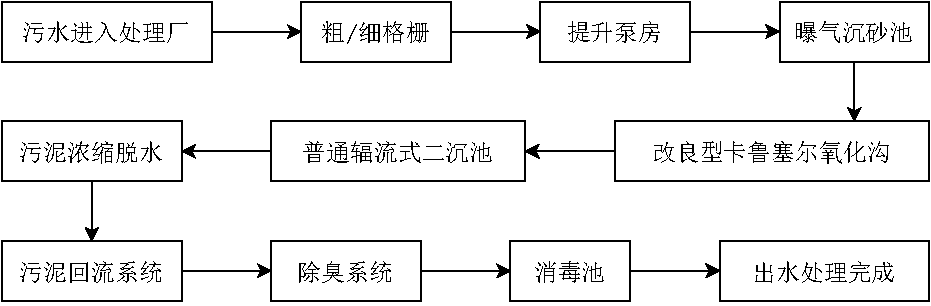
\includegraphics[width=0.92\textwidth]{figures/flowchart.drawio.pdf}
	% \begin{tikzpicture}[node distance=2cm, every node/.style={rectangle, draw, minimum width=3cm, minimum height=1cm, align=center}]
	%     \node (inlet) {污水进入处理厂};
	%     \node (coarse) [right=1.5cm of inlet] {粗格栅};
	%     \node (fine) [right=1.5cm of coarse] {细格栅};
	%     \node (pump) [right=1.5cm of fine] {提升泵房};
	%     \node (aeration) [below=1.5cm of pump] {曝气沉砂池};
	%     \node (oxidation) [left=1.5cm of aeration] {改良型卡鲁塞尔氧化沟};
	%     \node (settling) [left=1.5cm of oxidation] {普通辐流式二沉池};
	%     \node (thickening) [left=1.5cm of settling] {污泥浓缩};
	%     \node (recycle) [below=1.5cm of thickening] {污泥回流系统};
	%     \node (deodorization) [right=1.5cm of recycle] {除臭系统};
	%     \node (disinfection) [right=1.5cm of deodorization] {消毒池};
	%     \node (outlet) [right=1.5cm of disinfection] {出水处理完成};

	%     \draw[->] (inlet) -- (coarse);
	%     \draw[->] (coarse) -- (fine);
	%     \draw[->] (fine) -- (pump);
	%     \draw[->] (aeration) -- (oxidation);
	%     \draw[->] (oxidation) -- (settling);
	%     \draw[->] (recycle) -- (deodorization);
	%     \draw[->] (deodorization) -- (disinfection);
	%     \draw[->] (disinfection) -- (outlet);

	%     % Additional arrows for the S-shape layout
	%     \draw[->] (pump) |- (aeration);
	%     \draw[->] (thickening) |- (recycle);
	% \end{tikzpicture}
	\caption{城镇污水处理厂处理流程图}
	\label{fig:flowchart}
\end{figure}

\subsubsection{进出水质}
根据准备设计的城镇污水处理厂(日平均流量 $Q=35000$ m$^3$/d)的进水水质,我们在制定出水水质要求时优先选择更严格的地方标准,参考《城镇污水处理厂污染物排放标准》A标准(见表 \ref{tab:Pollutant discharge standards for urban sewage treatment plants})以及《四川省岷江、沱江流域水污染物排放标准》城镇污水处理厂污染物排放标准(见表 \ref{tab:Water pollutant discharge standards in the Minjiang and Tuojiang River basins of Sichuan Province})。这样的选择确保了城镇污水处理厂的出水能够满足地方环境保护要求。当地方标准无法明确规定时,我们将参考国家标准来确定出水水质要求。通过这种方法,我们能够确保排放的污水达到最高的环境质量标准,从而有效地保护周围水体和生态环境的健康。
但又考虑到本次城镇污水处理厂的设计地区并不在四川省岷江、沱江流域,综合考虑之下,本次设计会优先满足国家A标准,若是工艺优良,在能力之余则跟进满足地方标准。
以下是具体的进出水水质要求和标准:

\begin{table}[H]
	\centering
	\caption{进出水水质}
	\begin{tabular}{cccc}
		\toprule
		污染物   & 进水水质(mg/L) & 出水水质(mg/L) & 要求去除效率(\%) \\
		\midrule
		COD$\mathrm{_{C_r}}$ & 400   & 50    & 87.5  \\
		BOD$_5$  & 260   & 10     & 96.2 \\
		SS    & 280   & 10    & 96.4  \\
		NH$_4^+$-N\footnotemark & 35    & 5(8) & 85.7  \\
		TP    & 3     & 0.5   & 83.3  \\
		TN    & 45    & 15    & 66.7  \\
		\bottomrule
	\end{tabular}%
	\label{tab:in water}%
\end{table}%
\footnotetext{括号外数值为水温 $>12$ ℃时的控制指标,括号内数值为水温 $\leqslant 12$ ℃时的控制指标。}

\subsection{设计依据}
\subsubsection{法律法规}
\begin{enumerate}
	\item 《水污染防治行动计划》(2015.04);
	\item 《中华人民共和国环境保护法》(2015.01);
	\item 《中华人民共和国水污染防治法》(2008.06)。
\end{enumerate}

\subsubsection{参考规范及标准}
\begin{enumerate}
	\item 《室外排水设计规范》(GB 50014-2021);
	\item 《城镇污水处理厂污染物排放标准》(GB 18918-2002);
	\item 《建筑给水排水设计标准》(GB 50015-2019)
	\item 《四川省岷江、沱江流域水污染物排放标准》(DB 51/2311-2016);
	\item 《氧化沟活性污泥法污水处理工程技术规范》(HJ 578-2010)
	\item 《污水气浮处理工程技术规范》(HJ 2007-2010)
	\item 《给排水制图标准》GB/T50106-2001(2010 年);
	\item 《四川省建设工程工程量清单计价定额市政工程》(2020 年);
	\item 《关于印发城镇污水处理提质增效三年行动方案(2019-2021 年)的通知》。
\end{enumerate}



\newpage % 章节结尾换页